% =================================================
% 性学系列 · BDSM 与 Kink
% 共享基座见 common.tex
% =================================================
\documentclass[12pt,UTF8,openany]{ctexbook}
% =================================================
% common.tex —— 性学系列 共享基座
% 导言区 / 配色 / TikZ 库 / ctexset / C 列型 / 字体 / 书眉页码
% 各册 % =================================================
% common.tex —— 性学系列 共享基座
% 导言区 / 配色 / TikZ 库 / ctexset / C 列型 / 字体 / 书眉页码
% 各册 % =================================================
% common.tex —— 性学系列 共享基座
% 导言区 / 配色 / TikZ 库 / ctexset / C 列型 / 字体 / 书眉页码
% 各册 \input{common.tex} 引用
% =================================================
\usepackage[top=2.5cm,bottom=2.5cm,left=2.6cm,right=2.6cm,headheight=2.0cm]{geometry}
\usepackage{amsmath}
\usepackage{amssymb}
\usepackage{array}
\usepackage{tabularx}
\usepackage{multirow}
\usepackage{booktabs}
\usepackage{enumitem}
\usepackage{xcolor}
\usepackage{graphicx}
\usepackage{tikz}
\usetikzlibrary{positioning,calc,arrows.meta,shapes.geometric,matrix}
\definecolor{myblue}{HTML}{185FA5}
\definecolor{myblueL}{HTML}{E6F1FB}
\definecolor{mygreen}{HTML}{3B6D11}
\definecolor{mygreenL}{HTML}{C0DD97}
\definecolor{myteal}{HTML}{1D9E75}
\definecolor{myamber}{HTML}{854F0B}
\definecolor{myamberL}{HTML}{FAEEDA}
\definecolor{myred}{HTML}{A32D2D}
\definecolor{myredL}{HTML}{FCEBEB}
\definecolor{mypurple}{HTML}{534AB7}
\definecolor{mypurpleL}{HTML}{EEEDFE}
\definecolor{mycoral}{HTML}{D85A30}
\definecolor{mycoralL}{HTML}{FAECE7}
\definecolor{mypink}{HTML}{D4537E}
\definecolor{mypinkL}{HTML}{F4C0D1}
\definecolor{mypinkM}{HTML}{ED93B1}
\definecolor{mygray}{HTML}{888780}

% 字体
\setCJKfamilyfont{hei}{SimHei}
\newcommand{\myhei}{\CJKfamily{hei}}

% 书眉与页码（印刷友好：中文页眉 + 居中页码）
\usepackage{fancyhdr}
\pagestyle{fancy}
\fancyhf{}
\fancyhead[L]{\small\myhei 性学系列}
\fancyhead[R]{\small\leftmark}
\fancyfoot[C]{\small\thepage}
\renewcommand{\headrulewidth}{0.4pt}
\fancypagestyle{plain}{\fancyhf{}\fancyfoot[C]{\small\thepage}\renewcommand{\headrulewidth}{0pt}}
\fancypagestyle{empty}{\fancyhf{}\renewcommand{\headrulewidth}{0pt}}

% 行距（零基础易读，略松）
\linespread{1.3}

% 超链接：印刷友好（黑色，电子版仍可点击）
\usepackage[colorlinks,linkcolor=black,citecolor=black,urlcolor=black]{hyperref}

\ctexset{
  chapter/name={第,章},
  chapter/number={\arabic{chapter}},
  section/format=\Large\bfseries,
}

\newcolumntype{C}{>{\centering\arraybackslash}X}
 引用
% =================================================
\usepackage[top=2.5cm,bottom=2.5cm,left=2.6cm,right=2.6cm,headheight=2.0cm]{geometry}
\usepackage{amsmath}
\usepackage{amssymb}
\usepackage{array}
\usepackage{tabularx}
\usepackage{multirow}
\usepackage{booktabs}
\usepackage{enumitem}
\usepackage{xcolor}
\usepackage{graphicx}
\usepackage{tikz}
\usetikzlibrary{positioning,calc,arrows.meta,shapes.geometric,matrix}
\definecolor{myblue}{HTML}{185FA5}
\definecolor{myblueL}{HTML}{E6F1FB}
\definecolor{mygreen}{HTML}{3B6D11}
\definecolor{mygreenL}{HTML}{C0DD97}
\definecolor{myteal}{HTML}{1D9E75}
\definecolor{myamber}{HTML}{854F0B}
\definecolor{myamberL}{HTML}{FAEEDA}
\definecolor{myred}{HTML}{A32D2D}
\definecolor{myredL}{HTML}{FCEBEB}
\definecolor{mypurple}{HTML}{534AB7}
\definecolor{mypurpleL}{HTML}{EEEDFE}
\definecolor{mycoral}{HTML}{D85A30}
\definecolor{mycoralL}{HTML}{FAECE7}
\definecolor{mypink}{HTML}{D4537E}
\definecolor{mypinkL}{HTML}{F4C0D1}
\definecolor{mypinkM}{HTML}{ED93B1}
\definecolor{mygray}{HTML}{888780}

% 字体
\setCJKfamilyfont{hei}{SimHei}
\newcommand{\myhei}{\CJKfamily{hei}}

% 书眉与页码（印刷友好：中文页眉 + 居中页码）
\usepackage{fancyhdr}
\pagestyle{fancy}
\fancyhf{}
\fancyhead[L]{\small\myhei 性学系列}
\fancyhead[R]{\small\leftmark}
\fancyfoot[C]{\small\thepage}
\renewcommand{\headrulewidth}{0.4pt}
\fancypagestyle{plain}{\fancyhf{}\fancyfoot[C]{\small\thepage}\renewcommand{\headrulewidth}{0pt}}
\fancypagestyle{empty}{\fancyhf{}\renewcommand{\headrulewidth}{0pt}}

% 行距（零基础易读，略松）
\linespread{1.3}

% 超链接：印刷友好（黑色，电子版仍可点击）
\usepackage[colorlinks,linkcolor=black,citecolor=black,urlcolor=black]{hyperref}

\ctexset{
  chapter/name={第,章},
  chapter/number={\arabic{chapter}},
  section/format=\Large\bfseries,
}

\newcolumntype{C}{>{\centering\arraybackslash}X}
 引用
% =================================================
\usepackage[top=2.5cm,bottom=2.5cm,left=2.6cm,right=2.6cm,headheight=2.0cm]{geometry}
\usepackage{amsmath}
\usepackage{amssymb}
\usepackage{array}
\usepackage{tabularx}
\usepackage{multirow}
\usepackage{booktabs}
\usepackage{enumitem}
\usepackage{xcolor}
\usepackage{graphicx}
\usepackage{tikz}
\usetikzlibrary{positioning,calc,arrows.meta,shapes.geometric,matrix}
\definecolor{myblue}{HTML}{185FA5}
\definecolor{myblueL}{HTML}{E6F1FB}
\definecolor{mygreen}{HTML}{3B6D11}
\definecolor{mygreenL}{HTML}{C0DD97}
\definecolor{myteal}{HTML}{1D9E75}
\definecolor{myamber}{HTML}{854F0B}
\definecolor{myamberL}{HTML}{FAEEDA}
\definecolor{myred}{HTML}{A32D2D}
\definecolor{myredL}{HTML}{FCEBEB}
\definecolor{mypurple}{HTML}{534AB7}
\definecolor{mypurpleL}{HTML}{EEEDFE}
\definecolor{mycoral}{HTML}{D85A30}
\definecolor{mycoralL}{HTML}{FAECE7}
\definecolor{mypink}{HTML}{D4537E}
\definecolor{mypinkL}{HTML}{F4C0D1}
\definecolor{mypinkM}{HTML}{ED93B1}
\definecolor{mygray}{HTML}{888780}

% 字体
\setCJKfamilyfont{hei}{SimHei}
\newcommand{\myhei}{\CJKfamily{hei}}

% 书眉与页码（印刷友好：中文页眉 + 居中页码）
\usepackage{fancyhdr}
\pagestyle{fancy}
\fancyhf{}
\fancyhead[L]{\small\myhei 性学系列}
\fancyhead[R]{\small\leftmark}
\fancyfoot[C]{\small\thepage}
\renewcommand{\headrulewidth}{0.4pt}
\fancypagestyle{plain}{\fancyhf{}\fancyfoot[C]{\small\thepage}\renewcommand{\headrulewidth}{0pt}}
\fancypagestyle{empty}{\fancyhf{}\renewcommand{\headrulewidth}{0pt}}

% 行距（零基础易读，略松）
\linespread{1.3}

% 超链接：印刷友好（黑色，电子版仍可点击）
\usepackage[colorlinks,linkcolor=black,citecolor=black,urlcolor=black]{hyperref}

\ctexset{
  chapter/name={第,章},
  chapter/number={\arabic{chapter}},
  section/format=\Large\bfseries,
}

\newcolumntype{C}{>{\centering\arraybackslash}X}


\begin{document}

% ===== 封面 =====
\begin{titlepage}
\centering
\vspace*{1.5cm}
\begin{tikzpicture}
\draw[myblue,line width=2pt] (0,0) circle (1.2);
\node[text=white] at (0,0) {\myhei\zihao{3}性};
\end{tikzpicture}
\vspace{0.6cm}
\noindent\rule{\textwidth}{0.4pt}
\vspace{0.5cm}
\myhei\zihao{5} 性学系列\,·\,家庭健康科普\,·\,全五册
\vspace{2.5cm}
\myhei\zihao{0} BDSM 与 Kink\par
\vspace{1.2cm}
\itshape\zihao{3} 安全框架下的亲密表达\par
\vspace{5.2cm}
\noindent\rule{\textwidth}{0.4pt}
\vspace{0.5cm}
\zihao{5} 性学系列\,·\,\today
\end{titlepage}

% ===== 免责声明 =====
\begin{center}\zihao{5}\itshape
本书为家庭健康科普读物，内容力求科学严谨，但\textbf{不替代专业医生的诊断与治疗}。\\
涉及个人健康问题，请以正规医疗机构的检查与建议为准。\\
全书以安全、自愿、相互尊重为底色，尊重多元与个体差异。\par\end{center}
\clearpage

% ===== 如何使用本书 =====
\chapter*{如何使用本书}
\addcontentsline{toc}{chapter}{如何使用本书}
\noindent\textbf{性学系列共五册：}
\begin{itemize}[leftmargin=2em]
\item \textbf{A 性健康基础} —— 认知、同意、防护、STI、避孕总论（建议先读）
\item \textbf{B 亲密实践与技巧} —— 前戏、体位、高潮引导、呼吸与盆底
\item \textbf{C 男性性健康} —— 男性解剖、ED/自慰、绝育、不育
\item \textbf{D 女性性健康} —— 女性解剖、妇科、不孕、人流、避孕、孕期/更年期
\item \textbf{E BDSM 与 Kink} —— 安全框架下的亲密表达
\end{itemize}
\vspace{0.6em}
\noindent\textbf{建议阅读路径（零基础）：} 先通读 A 建立认知与安全底线 → 按需读 C 或 D 了解自己的身体 → 再读 B 学技巧 → 兴趣到了再读 E。每章末附有本章小结，便于快速回顾。
\clearpage

% ===== 目录 =====
\tableofcontents
\clearpage
\chapter{BDSM 与 Kink：安全框架下的亲密表达}
\label{chap:bdsm}

\section{一、BDSM 是什么}

\textbf{BDSM} = Bondage \& Discipline（束缚与纪律）+ Dominance \& Submission（主导与臣服）+ Sadism \& Masochism（施虐与受虐），是对一类\textbf{非传统亲密实践}的总称；圈内更宽泛的用词是 \textbf{kink（癖好）}。三个关键认知：

\begin{itemize}
  \item \textbf{不是"另一种性"，是亲密表达的谱系之一}。它与"普通性爱"不是替代关系，而是光谱上的不同位置。有人一辈子只玩轻 kink（眼罩、轻拍打、角色游戏），有人玩到窒息、医疗服从——都是正常范围。
  \item \textbf{DSM-5 的关键去病理化（2013 起）}：此前 APA 把"性施虐/受虐"列为 paraphilias（性偏好）；DSM-5 起把"性偏好（paraphilia）"与"\textbf{性偏好障碍（paraphilic disorder）}"区分开——\textbf{只有当偏好带来显著痛苦、或明显影响生活功能时才算障碍}。BDSM 本身不再被默认"是病"。
  \item \textbf{远比想象中普遍}：Indiana University 对 2021 名美国成年人的研究中——拍打 30\%、dom/sub 角色 22\%、束缚 20\%、鞭打 13\%；41 国 31.7 万人调查中约 20\% 用过眼罩/束缚。也就是说，"有 kink 元素"是\textbf{多数成年人的经验}，只是多数人一辈子只在私下进行、不告诉他人。
\end{itemize}

\section{二、常见形式：不是清单，是光谱}

Kink 不是一份清单，而是\textbf{光谱}。大致分三档（每档内组合差异极大，每个人不同）：

\begin{tabularx}{\textwidth}{lX}
\toprule
\textbf{强度} & \textbf{典型内容与主要风险点} \\
\midrule
Light（轻） & 角色游戏、眼罩、耳语、轻拍打、温柔束缚——主要风险是\textbf{情绪（aftercare）与隐私}。 \\
Medium（中） & 鞭打、温度（蜡烛/冰块）、体位控制、感官剥夺——注意\textbf{皮肤/软组织损伤、束缚过紧}。 \\
Deep（深） & 窒息、医疗服从、长时间束缚、多伙伴——\textbf{窒息、神经/血流、感染}，需要经验与准备。 \\
\bottomrule
\end{tabularx}

\vspace{0.5em}
\noindent\textbf{关键：} 三档之间没有绝对界限，"deep"不是"更厉害"，只是\textbf{风险类型不同}。多数人一辈子只在 light 到 medium 之间。

\section{三、安全框架：SSC 与 RACK}

BDSM 的安全不是"小心一点"，而是一套\textbf{可执行的协议}：

\begin{itemize}
  \item \textbf{SSC}：Safe（安全）、Sane（理智）、Consensual（自愿）——圈内最经典的三原则。
  \item \textbf{RACK}：Risk-Aware Consensual Kink（\textbf{知情风险}下的自愿 kink）——比 SSC 更精细，强调"双方都知道风险是什么、能承担、才做"。
\end{itemize}

无论用哪个框架，都落到\textbf{三个动作}：\textbf{事前谈判}（hard limits 绝对不做 / soft limits 视情况 / 想要什么 / 有无基础病如心血管·糖尿病·哮喘·癫痫·凝血问题）、\textbf{事中纪律}（安全词、节奏与观察、任何"不对"就停）、\textbf{事后关怀}（aftercare，见第六节）。

\section{四、五大风险与医学依据}

\subsection*{1. 窒息（最高危，单独列）}
\textbf{颈压}：颈动脉窦是颈动脉分叉处的压力感受器，受压会触发\textbf{颈动脉窦反射}——迷走神经兴奋，心率骤降、血压骤降。三型：
\begin{itemize}
  \item \textbf{心脏抑制型（迷走型）}：占 50--70\%，可致心率降至 40 次/分以下甚至短暂心脏停搏；
  \item \textbf{血管抑制型}：5--10\%，血压骤降；
  \item \textbf{中枢型（脑型）}：晕厥伴抽搐。
\end{itemize}
60 岁以上晕厥患者中 17.6\% 与颈动脉窦相关，70 岁以上达 25\%；常见触发为扼颈、勾肩、亲吻颈部、衣领过紧、颈部按摩。\textbf{口鼻阻塞}则导致脑缺氧。系统综述（2010，48 例 CiRCA 案例）显示：绝大多数颈压猝死其实\textbf{合并脑缺氧}（颈动脉血流完全阻断），纯反射单独致死罕见——但风险依然不可控。圈内共识：\textbf{新手不做颈压与窒息；若进行，必须有人全程在场}。高危人群：老年、动脉硬化、糖尿病、正在服降压/抗心律失常药、酒精影响后。

\subsection*{2. 束缚}
主要风险是\textbf{血液循环受阻}（远端发白/发紫、发凉）与\textbf{神经压迫}（腕管、尺神经、坐骨神经——出现"麻、木、针刺"立即松开）。四肢持续束缚\textbf{不建议超过 30--60 分钟}，其间观察颜色/温度/感觉。工具选择：软绳 $>$ 皮革 $>$ 金属，避免细绳勒进皮肤。

\subsection*{3. 疼痛与软组织损伤}
淤青（皮下出血）是\textbf{正常}，数周内消退。\textbf{警惕}：皮肤破损出血、大面积淤青不退、疼痛超一周——可能是深部组织损伤或凝血问题。糖尿病/凝血问题/正在用抗凝药者，深拍打需谨慎。

\subsection*{4. 情绪回落（sub drop / dom drop）}
高强度 BDSM 后，\textbf{双方}都可能经历 30 分钟到数小时的\textbf{情绪低谷}——低落、脆弱、想哭、疲惫。机制是\textbf{催产素、多巴胺、内啡肽在峰值后回落}。\textbf{不是"矫情"，是神经内分泌的正常反应}，处理见第六节 aftercare。

\subsection*{5. 传染}
任何涉及体液/共用器具的场景，感染风险与主流性行为一致；屏障工具（安全套/避孕套、dental dam）在 BDSM 里同样适用；共用器具前后清洗/换套。

\section{五、安全词：为什么需要、怎么设}

\textbf{为什么}：在高强度感官刺激、感官剥夺或主导-臣服角色下，"不"和"疼"可能\textbf{失效}——身体在"兴奋"与"疼痛"的信号会混淆，当事人可能本能地"忍着"，而对方无法分辨。安全词就是\textbf{一个事先约定的、在情境外、明确的停/降档信号}。

\textbf{怎么设}：
\begin{itemize}
  \item \textbf{红绿灯}（最常用）：\textcolor{mygreen}{绿} = 继续；\textcolor{myamber}{黄} = 慢一点/换个方向；\textcolor{myred}{红} = \textbf{立刻停}（不管进行到哪一步）。
  \item \textbf{水果词}（避免和"不"混淆）：预先约定两个词，如"菠萝 = 慢"、"芒果 = 停"——好处是"疼""不要"不会被误读。
  \item \textbf{纪律}：说了安全词，\textbf{无条件停下、检查、再谈}——这是 SSC 的底线。
\end{itemize}

\section{六、Aftercare（事后关怀）}

\textbf{是什么}：BDSM 结束后\textbf{一段刻意安排的关怀时间}，通常 30 分钟到数小时。\textbf{为什么}：OT/DA 峰值后回落，双方（dom 与 sub）都易进入情绪低谷（sub drop / dom drop），此时身体敏感、情感脆弱；aftercare 是给这段回落一个\textbf{"软着陆"}。\textbf{做什么}（按需求，不是清单）：温暖（毯子、拥抱）、补水吃点东西、轻声确认"你还好吗"、一起清理并慢慢离开场景、事后 24 小时内的正常关怀——不是"翻旧账"，而是把关系接回日常。\textbf{常见误区}：aftercare 只给 sub——\textbf{dom 也需要}，很多 dom 事后情绪回落同样明显。

\section{七、常见误区}

\begin{tabularx}{\textwidth}{lX}
\toprule
\textbf{误区} & \textbf{事实} \\
\midrule
"BDSM = 性变态" & DSM-5 起已区分"偏好"与"障碍"；只有带来显著痛苦/功能受损才算障碍。 \\
"痛苦 = 高潮" & 愉悦是\textbf{心理 + 生理 + 关系}多维的，不是单纯的痛。 \\
"只有特定性别/性取向才玩" & 所有性别和性取向都有 kink 玩家。 \\
"一定要用道具" & 眼神、耳语、节奏、呼吸都是 kink。 \\
"一定要玩很大" & 光谱上 light 完全够用，不必升级。 \\
"第一次就玩 deep" & 经验、信任、沟通是前提，deep 需要时间积累。 \\
\bottomrule
\end{tabularx}

\section{八、和主流性爱的关系}

\textbf{不是替代、不是升级、不是堕落}——是亲密表达的\textbf{一个维度}。你和伴侣可以一辈子只玩 light（角色游戏、眼罩、轻拍打），或只在特定场景玩，或完全不玩——都完全正常。\textbf{关键}：kink 是\textbf{加分项}，不是\textbf{必选项}。

\section{九、何时需要专业帮助}

当它变成\textbf{强迫性}（不做就难受、做就停不下来）；成为\textbf{唯一能唤起}的方式且明显影响关系；有\textbf{创伤史}、触发时反应剧烈并影响日常；或伴随\textbf{反复疼痛/损伤}且找不到原因——找\textbf{正规性医学科/心理科}，别把"圈内咨询师"当唯一渠道。

\section{十、红旗信号（立刻停下）}

\begin{itemize}
  \item 说了安全词，对方不停；
  \item 束缚超过 1 小时，远端发白/发紫；
  \item 颈部受压后头晕、视物模糊、心率异常；
  \item 皮肤大面积破损，或疼痛超过一周不退；
  \item 事后 24 小时情绪仍显著低落且无法自我调节。
\end{itemize}

\section{一页速查}

\begin{tabularx}{\textwidth}{lX}
\toprule
\textbf{项目} & \textbf{要点} \\
\midrule
安全框架 & SSC / RACK。 \\
事前 & hard/soft limits、基础病筛查。 \\
安全词 & 红绿灯或水果词；说了无条件停。 \\
窒息 & 新手不做颈压；若进行须有人全程在场。 \\
束缚 & 30--60 分钟上限；观察颜色/温度/感觉。 \\
Aftercare & 30 分钟到数小时；\textbf{双方都需要}。 \\
传染 & 屏障工具同样适用。 \\
就医 & 强迫性/唯一唤起/反复损伤/创伤史。 \\
\bottomrule
\end{tabularx}

\vspace{1em}
\noindent\textbf{要点：} BDSM 不是"另一种性"，是亲密表达的\textbf{一个维度}——\textbf{SSC/RACK + 安全词 + aftercare} 三件套到位，它就和任何亲密行为一样，可以既愉悦又安全。

\chapter{非常性爱：非主流亲密玩法}
\chapter{非主流亲密玩法：从"想知道"到"会玩"}
在"常规"之外，还有一大片常被统称"非主流亲密玩法"的领域——角色扮演、感官游戏（温度/食物）、轻度束缚、语言挑逗，乃至更深入的 kink。它们不是"变态"，而是亲密表达的\textbf{一个维度}；只是多数人没被正式教过，于是要么羞于尝试，要么凭感觉乱试。本章按"为什么、怎么开始、注意什么"把这些玩法摊开讲，供你按需取用。
\textbf{关键前提}：本章所有玩法都建立在第 1 章讲的\textbf{安全框架（SSC/RACK）+ 安全词 + aftercare}之上——\textbf{先同意、再尝试}；任何让你或对方不舒服的，\textbf{都可以不做}。
\subsection*{差异化实践的合理性}
多数人一辈子只在"轻档"（眼罩、轻拍打、角色扮演）之间；这不是"不够开放"，只是\textbf{舒适区}。真正阻碍尝试的往往不是能力，而是\textbf{两个念头}：\textbf{怕被看作"变态"}、\textbf{怕自己"不喜欢"才不敢试}。先澄清几点：
\begin{itemize}[leftmargin=2em,itemsep=0.3em]
  \item \textbf{别用别人的性观念来评价自己}——无论你们决定做什么，你们都是两个自愿的成年人。
  \item \textbf{"加一点不同"不等于"扭曲/恶心"的性爱}，它是给关系增添活力最常见的方式之一。
  \item \textbf{很多偏好要"试过才知道"}：你有时并不知道自己喜欢什么，直到试过。
  \item \textbf{不喜欢就停下}：知道不喜欢，就不要再做——"可以试"不等于"必须做"。
\end{itemize}
合理的尝试通常带来：更高的性趣与自信、把关系重新带出"例行公事"、更多的亲密连接。\textbf{但把"到没到高潮/玩没玩到位"当 KPI，反而最容易掉链子}——重点在过程与连接，不在达标。
\subsection*{玩法地图}
\textbf{怎么读}：按"门槛 + 关键注意"给每个玩法定档；同一玩法因力度、时长、人群不同，风险可能跨档——\textbf{看色更要看做法}。
\begin{tabularx}{\textwidth}{l X l}
\toprule
\textbf{玩法} & \textbf{要点} & \textbf{门槛/关键} \\
\midrule
感官剥夺（眼罩/耳塞/羽毛） & 放大触觉与想象 & 低；先建立信任 \\
温度与食物 & 冰/温/甜酸的刺激 & 中；\textbf{卫生与试温}是核心 \\
轻度束缚（bondage） & 限制 + 张力带来专注与顺从 & 中；留安全剪、避颈喉 \\
角色扮演（roleplay） & 换角色换剧情 & 低；先设计、越入戏越好玩 \\
恋物（fetish） & 对某物/某部位的迷恋 & 低；找到"你的触发点" \\
偷窥与裸露 & 把"被看/看"变一种玩法 & 中--高；同意与隐私第一 \\
语言挑逗（dirty talk） & 用语言点火 & 低；先谈界限 \\
非常规场所 & 环境本身带来刺激 & 中；安全与私密优先 \\
色情内容 & 借画面找点子 & 低；只是"选择"，不是"义务" \\
\bottomrule
\end{tabularx}
下面按玩法逐个展开。
\subsection*{沟通与尝试}
多数玩法卡住，不是能力问题，是\textbf{没聊清楚}。开始前，值得把这几件事谈明白：
\begin{itemize}[leftmargin=2em,itemsep=0.3em]
  \item \textbf{现实通常没幻想那么"顺"}：把期待说出口，问清对方是"真想做"还是"随口一提"。
  \item \textbf{只想"被欲望驱动"才做}：如果做某件事只是因为"怕不做他就走""朋友都试过"，那不如不做。
  \item \textbf{把"惊喜"换成"商量"，成功率更高}：很多人嘴上说喜欢，真被突然"惊喜"到会措手不及。开口邀请——"这是我想试的，我们可以试吗？"——比突然上演更好。
  \item \textbf{被拒绝很正常}：对方说"不"不等于"你不好"；你可以问清是"不喜欢"还是"还没准备好"，\textbf{再决定推进或换一种方式}。
  \item \textbf{提前定好"到哪一步、安全词是什么"}：玩之前把边界和退出方式说清楚，玩的时候才放松。
\end{itemize}
\textbf{关于"性幻想"}：把幻想当"菜单"而不是"考试"。可以和伴侣分享那些对方也能接受的部分；不必一次性倒完所有幻想（比如涉及第三方、前任的），\textbf{从对方接得住的开始}。读一些有情节描写的小说、回想让你心跳加速的经历、甚至聊聊彼此喜欢的场景，都是把"想"落到"玩"上的正常方式。常见的幻想类型（三人行/名人/认识的人/陌生人/顺从束缚/同性体验/被观看/公共场所）都可以当"点子"——\textbf{幻想是起点，能不能落地取决于双方的边界与准备}。
\subsection*{轻度束缚（bondage）}
束缚类玩法相当普遍，多数人幻想过被绑、被轻拍、被蒙眼、在挑逗中顺从。它的"有效"，来自\textbf{限制 + 张力}带来的专注与顺从感——\textbf{价值在氛围与心理，不在"疼"}。
\textbf{怎么做（要点）}：
\begin{itemize}[leftmargin=2em,itemsep=0.3em]
  \item \textbf{力度以"能塞下两指"为度}：目的是"束缚"，不是"勒断血流"；丝巾/丝带比粗糙材质更不磨皮肤。
  \item \textbf{先挑逗、再深入}：按摩、爱抚、在敏感区游移——被缚者的"快乐"掌握在另一方手里，顺从感由此而来。
  \item \textbf{可以交换角色}：被缚方"顺从"即可，不必全程发号施令。
\end{itemize}
\textbf{安全（务必）}：
\begin{itemize}[leftmargin=2em,itemsep=0.3em]
  \item \textbf{绝不把口/鼻塞住后把人单独留下}（窒息风险）；别用会压迫颈喉、阻碍呼吸的方式绑。
  \item \textbf{开始前定好"到第几步、安全词是什么"}；锁好门，避免被打断。
  \item 留一把\textbf{安全剪}；出现发麻、发紫、发凉，立即松开。
\end{itemize}
\subsection*{角色扮演（roleplay）}
换角色、换剧情，是消除"例行公事感"的常用手段——它让你们更专注彼此，也打破平时固定的"谁先发起"。
\textbf{怎么做（要点）}：
\begin{itemize}[leftmargin=2em,itemsep=0.3em]
  \item \textbf{先设计角色，越充分越不会笑场}：谁主导、谁顺从，医生对病人/师生/陌生人偶遇都行，编个小剧情。
  \item \textbf{把戏延伸到"卧室外"}：先扮演在酒吧相遇、用角色口吻发消息挑逗——越入戏，体验越好。
  \item \textbf{化装与道具}能加分，但"入戏"比"逼真"更重要。
\end{itemize}
\textbf{适合}：喜欢新鲜、有创造力、想把固定关系"重新开场"的伴侣。
\subsection*{恋物（fetish）}
"恋物"指对某个无生命物体或身体某部位的性迷恋——其实几乎每个人都有固定的"触发点"：特定的衣服、内衣、某双鞋、某个部位。它和"病"不是一回事，\textbf{多数人只是偏好，不需要"治疗"}。
\textbf{怎么做（要点）}：
\begin{itemize}[leftmargin=2em,itemsep=0.3em]
  \item \textbf{一起找"你的触发点"}：特定的衣物、配饰、部位、甚至气味。
  \item \textbf{把触发点变成"信号"}：在不预期的场合出现，往往是高效的"开场"。
  \item \textbf{只有当"缺了它就无法进行"时才需要正视}——这很少见，多数是偏好而非障碍。
\end{itemize}
\subsection*{偷窥与裸露（voyeurism / exhibitionism）}
"被看"或"看对方"对很多人都是兴奋点。这不一定指真在公众场合，更多是\textbf{把"通常被隐藏的行为"稍微公开一点}——用镜子、镜头、或"可能被人看到"的紧张感。
\textbf{怎么做（要点）}：
\begin{itemize}[leftmargin=2em,itemsep=0.3em]
  \item \textbf{镜子}：在上方位时放一面镜子，能看清角度、也能放大体验。
  \item \textbf{镜头}：自拍/录像、对着镜子做——"被观看感"是核心；\textbf{注意隐私}，用不联网的设备、拍完即删或加密。
  \item \textbf{"半公开"的紧张感}本身就是刺激：留一盏灯、开着窗帘——"可能被看到"比"真被看到"更带感，也更安全。
\end{itemize}
\textbf{安全}：偷窥类玩法的底线是\textbf{双方同意}——"被看"的一方有权随时叫停；涉及第三方真实观看时，\textbf{隐私与同意}是第一优先。
\subsection*{温度、食物与感官}
温度与食物质感（甜、酸、冰、温）是低门槛的感官玩法，但\textbf{卫生是硬底线}：
\begin{itemize}[leftmargin=2em,itemsep=0.3em]
  \item \textbf{温度}：冰块/体温蜡烛可先在手背试温；\textbf{别用普通蜡烛}（会烫伤），太冷/太烫都先降档。
  \item \textbf{食物}：草莓、香蕉、融化的巧克力等可涂抹、舔食；\textbf{避免过甜/过酸/过冷直接进入}（阴道与黏膜敏感），异物要\textbf{可取出}、别太尖。
  \item \textbf{口腔}：口交前避免辛辣/过冷/酒精；\textbf{口腔有伤口时暂缓}（黏膜破损增加 STI 传播风险，见 A 册）。
  \item \textbf{通用}：能放进嘴的东西才放身体；用后清洁；\textbf{不要"什么都往里塞"}（A 册经验法则）。
\end{itemize}
\subsection*{非常规场所}
环境本身就能带来刺激——海滩、户外、酒店阳台。它的核心是\textbf{新奇 + 可能被发现的紧张感}，但\textbf{安全和私密永远优先}：
\begin{itemize}[leftmargin=2em,itemsep=0.3em]
  \item \textbf{选地}：偏僻、有遮挡、人少；避开小孩多的海滩、公共步道、泳池旁。
  \item \textbf{卫生}：户外有沙/尘，\textbf{异物要可取出}；水中/沙中先清洁。
  \item \textbf{温度与体能}：户外风大易冷，注意保暖与时间。
  \item \textbf{安全底线}：乐趣在于"可能被发现的紧张"，不是"真的走投无路"——\textbf{先确认能随时退出}。
\end{itemize}
\subsection*{性玩具}
振动器、假阴茎、肛塞、阴茎圈、内用球等都是\textbf{性爱的延伸，不是替代}——用来找敏感区、增加刺激，\textbf{不必为此羞耻}，但也不是"必需品"。
\begin{itemize}[leftmargin=2em,itemsep=0.3em]
  \item \textbf{选对再买}：振动按摩器（柱状振动）、假阴茎（棒状）、肛塞（带底座）、阴茎圈（延时用）等，\textbf{先想清用途再选}（详见 B 册第 16 章）。
  \item \textbf{卫生}：用前用后清洗；\textbf{不要共用}（传播细菌与 STI）；多孔材质更易藏菌。
  \item \textbf{别当"长期替代"}：玩具是"加法"，不是把伴侣换掉。
\end{itemize}
\subsection*{语言挑逗（dirty talk）}
用语言点火——说你们之间"能接受的尺度"内的话，或描述正在发生/即将发生的画面。它能让"在场"的人提前进入状态，也能远程使用（语音/文字）。
\begin{itemize}[leftmargin=2em,itemsep=0.3em]
  \item \textbf{先谈界限}：你们能接受的"尺度"到哪，\textbf{别拿对方的"性趣"开玩笑}。
  \item \textbf{描述感受与欲望}比"念台词"更自然——说"我想要…""你刚才让我…"。
  \item \textbf{远程也适用}：电话/语音/文字挑逗，是把"亲密"延伸到全天的低成本方式。
  \item \textbf{对方笑场/不接}，可能是尺度不匹配——\textbf{降档或换词}，别硬推。
\end{itemize}
\subsection*{色情内容的角色}
色情片/图/文是"找点子"的工具之一，不是"教材"、更不是"义务"：
\begin{itemize}[leftmargin=2em,itemsep=0.3em]
  \item \textbf{它只是"选择"}：不喜欢就不必看，不必为了"合群"而看。
  \item \textbf{把它当"菜单"}：看画面找点子、学个节奏，\textbf{别把现实当表演}（时长、镜头、节奏都是剪辑/设计的）。
  \item \textbf{别拿它当"标准"}：多数影片为镜头与时长\textbf{省略前戏与沟通}——这正是很多误会的来源（A 册已强调）。
  \item \textbf{双方尺度可能不同}：一方觉得刺激、一方觉得"太"，是正常差异，\textbf{谈清楚就行}。
\end{itemize}
\subsection*{常见问答（精选）}
\begin{itemize}[leftmargin=2em,itemsep=0.5em]
  \item \textbf{带个振动器上床，会不会"不礼貌"？} 不会——只要双方同意。它常是"帮助"而非"替代"；\textbf{声音与节奏可先商量}，别突然"上机器"。
  \item \textbf{对方没让我到高潮，我能自己用玩具吗？} 可以，\textbf{但用"共享"的方式说}（"这个感觉不错，你帮我试试？"），比"你不行"更容易被接受。
  \item \textbf{我说下流话时对方笑了，算冒犯吗？} 可能尺度不匹配——\textbf{问清是"好笑"还是"不习惯"}，然后降档或换词。
  \item \textbf{我想"惩罚"对方，跟性有关吗？} 看动机：若是想"在床上主导/掌控"，那就是玩法；若是把情绪带进床，先处理情绪。
  \item \textbf{能"多变态"？} 在\textbf{双方同意 + 安全}的范围内都可以；\textbf{超出舒适区就先停}，不必"忍过去"。
\end{itemize}
\subsection*{可尝试的项目（分级）}
\textbf{按"轻 → 中 → 深"给一份可挑的菜单}（从你们接得住的开始，别一次上齐）：
\begin{itemize}[leftmargin=2em,itemsep=0.3em]
  \item \textbf{轻档}：眼罩 + 耳语；角色互换；读一段有情节的文字给对方；换一个新姿势；留一盏灯。
  \item \textbf{中档}：轻度束缚（丝巾）；温度/食物感官；dirty talk 一段；远程挑逗一次。
  \item \textbf{进阶}：角色扮演一整套（含卧室外）；恋物触发点；镜头/镜子；换一个新场所。
\end{itemize}
\textbf{原则}：一次只加一样，复盘"哪个最舒服、下次想改什么"，再往上走。
\subsection*{本章小结}
\begin{itemize}[leftmargin=2em,itemsep=0.3em]
  \item \textbf{非主流玩法 = 亲密的一个维度}，不是"变态"，也不是"义务"。
  \item \textbf{先聊再试}：边界、安全词、"到哪一步"先说清楚。
  \item \textbf{把"惊喜"换成"商量"}，成功率更高。
  \item \textbf{每个玩法的底线 = 双方同意 + 安全}；\textbf{能随时退出}比"玩到位"更重要。
  \item \textbf{卫生是硬底线}：食物/温度/场所/异物，先想"干净/可取出/能退出"。
  \item \textbf{一次只加一样}，复盘再往上走；\textbf{不喜欢就停}，不"忍"。
  \item \textbf{参考}：道具细节见第 3 章 Kink 安全进阶；束缚/口球/乳夹等专项指南见后文。
\end{itemize}

\chapter{Kink安全进阶：从SSC到PRICK，身体极限与aftercare}

\begin{center}
\myhei\large 进阶的关键不是"更猛"，而是"更懂边界、更会收尾"
\end{center}

\section{从 SSC 到 PRICK：框架的演进}
\begin{itemize}[leftmargin=2em,itemsep=0.3em]
  \item \textbf{SSC（Safe, Sane, Consensual）}：安全、理性、知情同意——\textbf{入门底线}，任何玩法的前提。
  \item \textbf{PRICK（Personal, Respectful, Informed, Consensual, Kinky）}：更强调\textbf{个人化 + 相互尊重}，适合\textbf{长期、深入}的关系。
  \item \textbf{核心没变}：\textbf{同意可以撤回}、\textbf{双方都自愿}、\textbf{风险被提前告知}——框架升级只是"更细致"，不是"更放纵"。
\end{itemize}

\section{风险分级（绿 / 黄 / 红）}
\begin{tabularx}{\textwidth}{X X}
\toprule
\textbf{级别} & \textbf{典型} \\
\midrule
绿（低） & 感官剥夺（眼罩）、轻抚、温度变化（体温蜡烛）、语言游戏 \\
黄（中） & 束缚（绳索/皮带）、拍打、蜡烛（需控制温度）、感官过载 \\
红（高） & 体压（breath play）、针刺、低温/高温、体位倒挂——\textbf{需经验 + 装备 + 备用方案} \\
\bottomrule
\end{tabularx}
\par\smallskip
\textbf{原则}：\textbf{从绿开始、逐级升}；\textbf{黄级要"备胎"}（备用工具/退出方式）；\textbf{红级要"双人 + 经验"}，别一个人"试"。

\section{Kink 道具与玩法分类总览（一张地图）}

\textbf{怎么读这张表}：把"道具/玩法"按\textbf{风险类型}分类，而不是按"高级/低级"。绿=低、黄=中、红=高（与上一节风险分级一致）。同一玩法\textbf{因力度、时长、人群不同}，风险可能跨档——\textbf{看"色"更要"看做法"}。

\begin{tabularx}{\textwidth}{l X l X}
\toprule
\textbf{分类} & \textbf{典型道具/玩法} & \textbf{风险} & \textbf{入门建议} \\
\midrule
感官剥夺 & 眼罩、耳塞、羽毛、感官刷 & 绿 & \textbf{低门槛}，适合第一次；\textbf{先建立信任}，别"突然从背后" \\
温度 & 体温蜡烛、冰块、加热/冷藏器具 & 绿--黄 & \textbf{先涂手背试温}；\textbf{别用普通蜡烛}（会烫伤） \\
束缚 & 绳索、皮带、手铐脚镣、分腿器、床上秋千、八爪椅 & 黄 & \textbf{留安全剪}、\textbf{能塞两指}、\textbf{避颈喉}、每 20--30 min 活动 \\
疼痛/拍打 & 软拍、鞭、指尖、电极(electro) & 黄--红 & \textbf{避脊柱/肾区/关节}、\textbf{从轻重开始}、\textbf{问"还要吗"} \\
夹持 & 乳夹、趾夹、唇夹（见专项） & 黄 & \textbf{旋钮式/小号}、单点\textbf{不超过 30 min}、取下看红印 \\
口含/呼吸 & 口球（见专项）、颈压(breath play) & 黄--红 & \textbf{第二人在场}；\textbf{颈压别单独做}、出现头晕/发紫立刻停 \\
角色扮演 & 台词、服装、场景、小道具 & 绿 & \textbf{低门槛}；\textbf{先设计角色}，越入戏体验越好 \\
侵入/深度刺激 & 肛塞、G 点棒、电刺激、医疗服从 & 黄--红 & \textbf{足量润滑}、\textbf{循序渐进}、\textbf{医疗类需更多经验与准备} \\
\bottomrule
\end{tabularx}

\vspace{0.5em}
\noindent\textbf{选道具的三条通用原则}：
\begin{itemize}[leftmargin=2em,itemsep=0.3em]
  \item \textbf{从绿开始、逐级升}：第一次别上"黄/红"；\textbf{信任与沟通}是比道具更重要的"道具"。
  \item \textbf{材质优先}：\textbf{医用硅胶/不锈钢}优于软胶/塑料；\textbf{避多孔材质}（易藏菌，肛用/共用尤甚）。
  \item \textbf{可逆、可退出}：\textbf{快拆}、\textbf{能随时停下}的设计，比"更刺激"更重要。
\end{itemize}

\subsection*{首次体验渐进路径（light $\to$ medium $\to$ deep）}
\begin{itemize}[leftmargin=2em,itemsep=0.3em]
  \item \textbf{第一次（light）}：\textbf{眼罩 + 耳语 + 轻抚 + 温柔束缚}（软绳/皮带、\textbf{不勒}）；目标不是"玩大"，而是\textbf{建立信任与节奏}；时长\textbf{30--60 min} 足够。
  \item \textbf{进阶（medium）}：在 light 基础上加\textbf{温度}（体温蜡烛）、\textbf{轻拍打}、\textbf{乳夹/趾夹}、\textbf{口球}（\textbf{第二人在场}）；每次都\textbf{复盘}"哪个最享受、下次调整什么"。
  \item \textbf{深入（deep）}：\textbf{颈压}、\textbf{长时间束缚}、\textbf{电极/医疗服从}、\textbf{多伙伴}——\textbf{需要经验 + 信任 + 装备 + 备用方案}，\textbf{别第一次就上}，\textbf{红级"双人"}是底线。
\end{itemize}

\noindent\textbf{要点：}道具是\textbf{放大器}，不是\textbf{开关}——\textbf{先有信任与沟通，再谈工具}；\textbf{从绿开始、逐级升}，比"一次玩到位"更可持续。

\section{常见玩法安全要点}
\begin{itemize}[leftmargin=2em,itemsep=0.3em]
  \item \textbf{绳索/束缚}：\textbf{别勒太紧、别压同一处过久}；\textbf{留剪刀/安全剪}在身边（意外时 10 秒内能解开）；\textbf{肩胛骨以下}（避免颈/喉）。
  \item \textbf{温度（蜡烛/冰块）}：\textbf{专用体温蜡烛}（熔点约 37$^\circ$C），\textbf{先涂手背试温}；\textbf{别用普通蜡烛}（会烫伤）；\textbf{避开破损皮肤}。
  \item \textbf{体压（breath play / 边缘呼吸）}：\textbf{高风险}——\textbf{别单独做}、\textbf{别"数到 10"}、\textbf{出现头晕/发紫立刻停}；\textbf{不是"忍一忍"的游戏}。
  \item \textbf{拍打/抽打}：\textbf{避脊柱、肾区、关节}；\textbf{用前确认皮肤无伤}；\textbf{力度从"轻"开始}，问"还要吗"比"猜"靠谱。
  \item \textbf{感官（眼罩/羽毛）}：\textbf{低门槛}，但\textbf{别"突然从背后"}（失去视觉时"方向感"也丢了）；\textbf{先建立信任}。
  \item \textbf{咬夹/夹子类（乳头夹 nipple clamp）}：\textbf{别用太大力}、\textbf{别夹同一处超过 30\,min}（皮肤缺血）；\textbf{避开破损/敏感过敏区}；\textbf{用后消毒+检查红印/淤青}。
\end{itemize}

\subsection*{束缚/分腿器（bondage / leg spreader）专项指南}

\textbf{是什么}：用绳、带、锁扣把手脚固定/约束的器具——图中这种是\textbf{手脚捆绑器}（绑带 + 锁扣，\textbf{把手腕/脚踝捆在一起}，限制动作、放大"被束缚"的顺从感）。有的款带分腿撑开功能，但\textbf{这张图主要是捆绑手腕脚踝}。同类还有\textbf{床柱吊绳、跪凳（kneeling bench）、手铐脚镣、分腿器}等。

\begin{center}
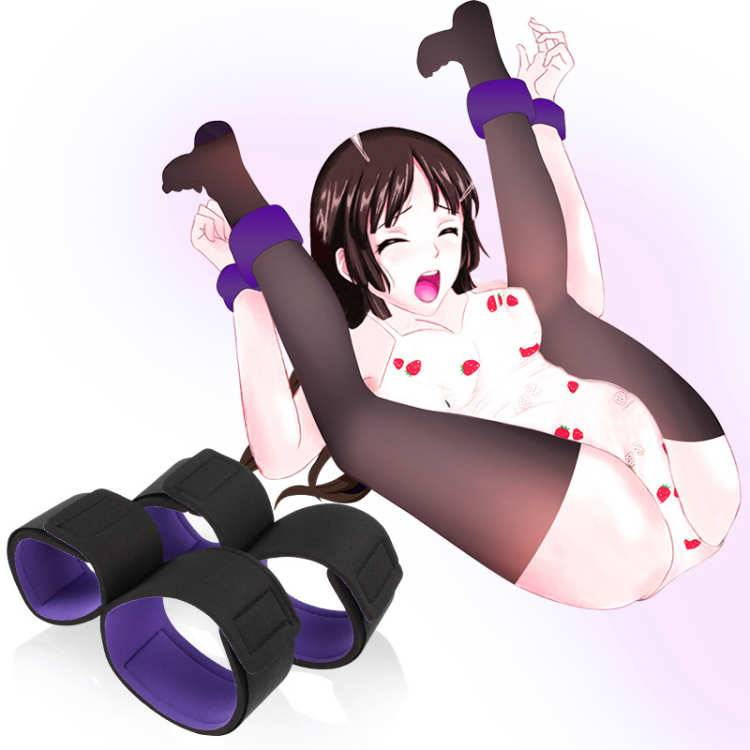
\includegraphics[width=0.42\textwidth]{images/fig_leg_spreader.jpg}\\
{\footnotesize 图：手脚捆绑器实物——绑带 + 锁扣结构，\textbf{把手腕/脚踝捆在一起}，属束缚类（bondage）。\textbf{核心风险是"血液循环 + 神经压迫"}，不是"疼不疼"。选型看\textbf{绑带软硬（选有衬垫的软带）、锁扣是否易解（带快拆/安全扣）、角度可调}（别选"死角度、松不得"的）。}
\end{center}
\par\smallskip

\noindent\textbf{使用要点（束缚类的安全底线）}：
\begin{itemize}[leftmargin=2em,itemsep=0.3em]
  \item \textbf{别勒太紧}：以"能塞进两指"为准——太紧会\textbf{压迫血管/神经}，出现\textbf{发麻、发紫、发凉、针刺感}要\textbf{立刻松}。
  \item \textbf{别压同一处过久}：同一部位束缚\textbf{不超过 20--30\,min}，\textbf{定时活动/松一松}，避免压疮/神经损伤。
  \item \textbf{避开颈/喉}：手/脚束缚\textbf{尽量在肩胛骨以下、膝盖以下}，\textbf{颈部}风险最高（压迫颈动脉/气道）。
  \item \textbf{留安全剪}：\textbf{一把快剪/安全剪随身}，意外时 10 秒内能解开；\textbf{别用"只有钥匙才能开"的锁}当入门款。
  \item \textbf{设安全词 + 保持能沟通}：束缚后\textbf{仍要能说话/摇铃/拍地}表达"停"；\textbf{别选"完全静音 + 不可动"的组合}当第一次。
  \item \textbf{皮肤检查}：有伤、湿疹、皮肤薄的人\textbf{先别束缚}该部位；\textbf{取下来看红印}（正常消退；\textbf{淤青/破皮/持续麻木}要留意）。
  \item \textbf{别在酒精/睡意下做}：痛觉和警觉都降低，\textbf{力度和时长容易失控}。
\end{itemize}

\noindent\textbf{要点}：束缚/分腿器 = \textbf{限制 + 张力}；\textbf{能塞两指/避颈喉/留安全剪/每 20--30 分钟活动/取下来看红印}——记住这五点，入门就稳。

\subsection*{门上秋千 / 八爪椅（固定类 furniture bondage）专项指南}

\textbf{是什么}：把"束缚"从"用手/脚"升级到\textbf{整个人被固定住}的家具级道具——
\begin{itemize}[leftmargin=2em,itemsep=0.3em]
  \item \textbf{门上秋千（door swing / door swing chair）}：\textbf{挂在门框上的秋千椅}，人坐上去、身体被安全带/带子固定，可\textbf{前后荡、分腿、抬升}，强调"被吊起来 + 顺从 + 体位辅助"。
  \item \textbf{八爪椅（octopus chair / 多带束缚椅）}：\textbf{带多条可调节带子的束缚椅}，像"八爪鱼"一样把手、臂、腿、躯干\textbf{各自独立固定}，松紧可调、角度可调，用于\textbf{束缚玩法 + 角色扮演 + 体位辅助}。
\end{itemize}
两者和前面的"分腿器/口球"差别：那些是\textbf{局部道具}，这两个是\textbf{全身固定的家具}——\textbf{束缚面积大、时间长、风险点更多}（承重、安全带、血液循环）。

\begin{center}
\fbox{\parbox{0.7\textwidth}{\centering 图位预留：门上秋千 + 八爪椅实物。待配图。}}
\end{center}
\par\smallskip

\noindent\textbf{使用要点（全身固定类的安全底线）}：
\begin{itemize}[leftmargin=2em,itemsep=0.3em]
  \item \textbf{先确认承重/安装}：门上秋千\textbf{挂前确认门框承重}（实木门框优于空心门框）、\textbf{挂钩/卡扣是快拆式}（一扣就开，别用只能慢慢松的螺丝）。八爪椅\textbf{确认椅架稳固、带子不脱扣}。
  \item \textbf{安全带要留"能呼吸 + 能活动"的余量}：坐上去\textbf{能正常呼吸、能轻微活动四肢}，别勒到\textbf{发麻/发紫/憋气}。
  \item \textbf{带子/绳别压同一处过久}：同一部位\textbf{不超过 20--30\,min}，\textbf{定时松一松}；\textbf{多带款}（八爪椅）注意\textbf{手腕/肘窝/腘窝/踝}这些\textbf{神经走行处}别压太死。
  \item \textbf{别荡太猛 / 别抬太高}（门上秋千）：\textbf{晃得越快越难自主下来}，\textbf{高度以"脚能着地或有人接"为准}，别吊到\textbf{完全离地、无人接}的高度。
  \item \textbf{留"自救/被救"的通道}：\textbf{快拆扣 + 旁边有人}是底线；\textbf{别用"只能钥匙开"的锁}当入门；\textbf{设安全词 + 保持能沟通/拍地/摇铃}。
  \item \textbf{别在酒精/睡意下用}：痛觉和警觉都降低，\textbf{被固定住的时长和力度容易失控}——\textbf{清醒状态}才安全。
  \item \textbf{取下来后看皮肤}：\textbf{红印正常消退}；\textbf{淤青/破皮/持续麻木}要留意，反复出现要查\textbf{神经/血管}。
\end{itemize}

\noindent\textbf{要点}：门上秋千/八爪椅 = \textbf{全身固定 + 张力}；\textbf{承重/快拆/留呼吸余量/别压神经处/留被救通道}——这五点缺一条，就\textbf{别第一次就全身固定}。

\subsection*{口球（ball gag）专项指南}

\textbf{是什么}：一个\textbf{软球（硅胶/橡胶）含在口中 + 一条系带/绳绕到脑后固定}，让含者\textbf{说不出话 + 微微有"含着东西"的紧张/失禁感 + 被束缚的顺从感}。它是 BDSM 里\textbf{偏高风险}的道具（接近 breath play）——因为球可能移位、堵住气道，\textbf{安全要求比前面几类都高}。

\begin{center}
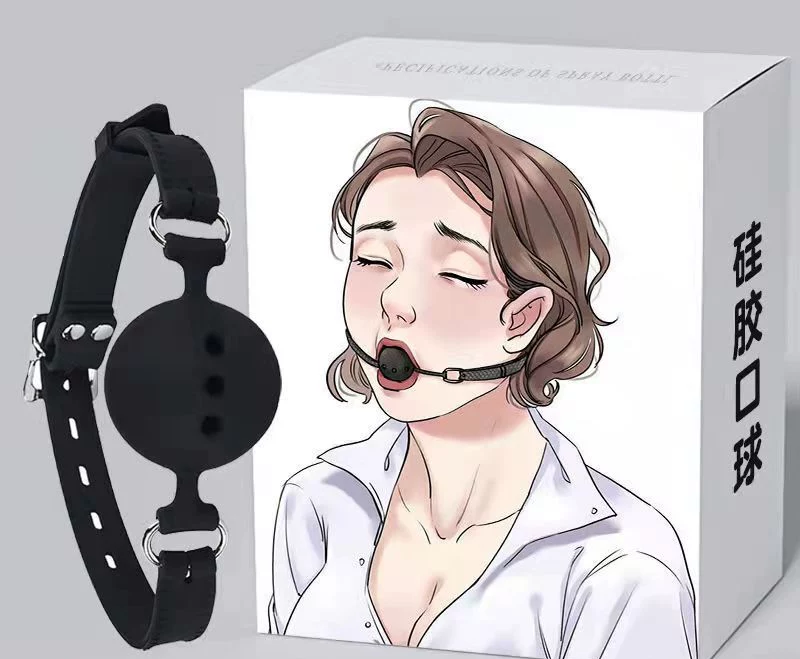
\includegraphics[width=0.42\textwidth]{images/fig_ball_gag.png}\\
{\footnotesize 图：口球（ball gag）实物——\textbf{黑色、球较大、两侧各一个小圆环，两环间一条可调节长度的皮带}（调松紧、绕脑后固定）。这类"球 + 圆环 + 皮带"造型在 Kink 语境里更强调\textbf{顺从/装饰感}，不只是"含个球"。注意：\textbf{球较大}时\textbf{安全要求更高}（易卡喉、误吞）——\textbf{入门先选软硅胶小球、系带可快拆}，\textbf{别一上来就用大球款}。}
\end{center}
\par\smallskip

\noindent\textbf{使用要点（高风险，安全优先）}：
\begin{itemize}[leftmargin=2em,itemsep=0.3em]
  \item \textbf{球要软、别太大}：选\textbf{硅胶软球、小尺寸}——硬球/大球\textbf{易卡喉、伤牙、堵住气道}。
  \item \textbf{必须有第二人在场}：口球\textbf{不是"独自玩"的道具}——万一球移位/含不住/误吞，\textbf{旁边必须有人能立刻取出来}。
  \item \textbf{系带/绳别太紧、留能呼吸的缝}：\textbf{能正常呼吸、能吞咽唾液}为准；\textbf{选带快拆的}（一扯就开，别用死结/钥匙锁）。
  \item \textbf{含的时间别太久}：下颌会酸、唾液增多；\textbf{每隔一会儿取出来活动一下}，别"含着一动不动半小时"。
  \item \textbf{有这些情况别用}：\textbf{吞咽困难、哮喘、气道过敏、牙/颌关节问题、醉酒/半睡}——误吞/窒息风险高。
  \item \textbf{别在完全无意识下用}：\textbf{半昏迷/深度醉酒}时含口球，\textbf{误吞风险}上升——\textbf{清醒状态下}用才安全。
  \item \textbf{取下来后别硬拽}：\textbf{沿原路慢慢取出}，检查口腔/牙齿有无压痕；\textbf{球每次用后清洗消毒}（含过唾液，多孔/软胶易藏菌）。
\end{itemize}

\noindent\textbf{要点}：口球 = \textbf{说不出话 + 束缚感}；\textbf{球软且小 / 第二人在场 / 留呼吸缝 / 别含太久 / 别半昏迷下用}——这五点是安全底线，\textbf{缺了任何一条就别玩}。

\subsection*{咬夹类（乳夹 / 乳头夹 / nipple clamp）专项指南}

\textbf{是什么}：金属（不锈钢/合金）或塑料夹，两瓣咬合，夹住乳头、耳垂、脚趾、唇缘等敏感点，靠\textbf{持续压迫 + 微痛感}放大快感。日常简称"乳夹"，医学/BDSM 语境称"乳头夹"或英文 nipple clamp。常见款式分两大类：\textbf{咬合式}——\textbf{弹簧式}（自动开合）、\textbf{旋钮式}（力度可调）、\textbf{松紧带式}（软质），靠\textbf{持续压迫}产生刺激；以及\textbf{环式/吊坠式}——上端是\textbf{可调大小的环}（套住乳头），下垂\textbf{链条或多种造型吊饰}（铃铛、水滴、圆珠等），靠\textbf{牵拉 + 晃动}产生刺激，通常更柔和、可长时间佩戴。

\begin{center}
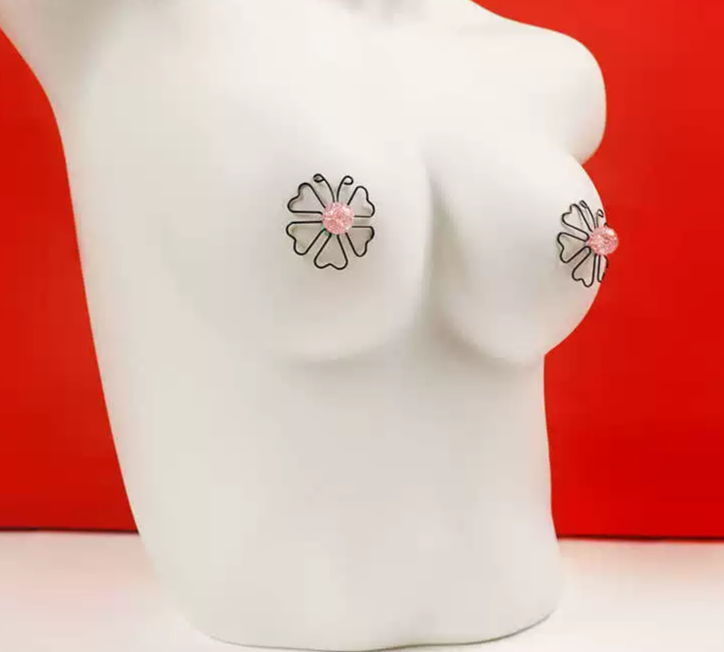
\includegraphics[width=0.32\textwidth]{images/fig_nipple_clamp.png}\\
{\footnotesize 图：乳夹（nipple clamp）实物——花瓣/蝴蝶形装饰款，两瓣咬合夹住乳头。市售乳夹\textbf{种类繁多}：功能型有弹簧式/旋钮式/松紧带式（力度可控）；\textbf{装饰型}常有蝴蝶、花瓣、爱心、皇冠、铃铛、羽毛等造型（如本图的黑色花瓣款），既夹持又兼具视觉。选型时"力度可调 + 夹口圆润不硌 + 装饰安全（无尖角）"三者兼顾，首次选\textbf{旋钮式/小号}。}
\end{center}
\par\smallskip

\begin{center}
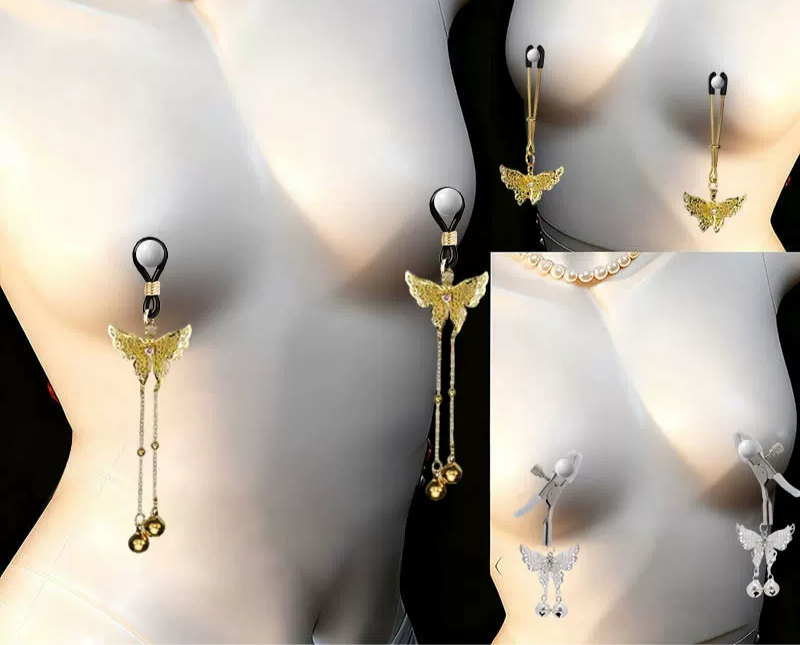
\includegraphics[width=0.42\textwidth]{images/fig_nipple_clamp_ring.png}\\
{\footnotesize 图：\textbf{环式/吊坠式}乳夹——上端为\textbf{可调大小的橡胶/硅胶环}，套住乳头；下垂\textbf{链条或多种造型吊饰}（铃铛、水滴、圆珠等）。与咬合式靠"压迫"不同，它靠\textbf{牵拉 + 晃动}产生刺激，\textbf{更柔和、可长时间佩戴}；吊饰随动作摆动，兼具\textbf{视觉与声音（铃铛）}效果。选型时环要\textbf{弹性适中、大小可调}（过紧易缺血、过松会脱落），吊饰\textbf{选无尖角、重量适中}（太重会牵拉疼痛）。}
\end{center}
\par\smallskip

\begin{center}
\footnotesize
\begin{tabularx}{\textwidth}{l X X}
\toprule
\textbf{维度} & \textbf{说明} & \textbf{选择建议} \\
\midrule
材质 & 不锈钢（可加热/冷藏）/ 塑料（软、入门）& 入门选\textbf{塑料或硅胶套}（金属硬、易夹伤）；进阶选\textbf{不锈钢} \\
尺寸 & 夹口宽度 1--2\,cm & \textbf{先选小号}（夹口 1\,cm 左右），别一上来就"大号" \\
开口/松紧 & 弹簧式（自动开合）/ 旋钮式（可调）/ 松紧带式 & \textbf{旋钮式最安全}（力度可调）；弹簧式省力但\textbf{力度不易控制} \\
温度 & 可加热（40--50$^\circ$C）/ 冷藏 & 温度玩法\textbf{别太热}（先涂手背试温）；\textbf{别直接用沸水} \\
\bottomrule
\end{tabularx}
\end{center}

\noindent\textbf{使用流程（逐步）}：
\begin{enumerate}[leftmargin=2em,itemsep=0.2em]
  \item \textbf{清洁}：温水 + 中性洗涤剂清洗，\textbf{首次使用前酒精/专用消毒}（去除工业残留）。
  \item \textbf{消毒后晾干}：别用湿巾反复擦（残留刺激）。
  \item \textbf{定位}：夹在\textbf{乳头/乳晕边缘}（避开乳晕正中心，太敏感易刺痛）；也可夹\textbf{耳垂、唇缘、脚趾、手背内侧}。
  \item \textbf{力度}：\textbf{先轻夹 1--2\,min}，让对方适应；\textbf{问"还要吗？"再加重}；\textbf{别用"越紧越好"思路}。
  \item \textbf{时间}：单点\textbf{不超过 30\,min}（皮肤缺血/微血管淤血）；\textbf{多点轮换}（左右乳头交替、夹/松交替）比"死夹一个点"更舒服。
  \item \textbf{取下}：缓慢松夹、\textbf{别猛拉}（皮肤微粘/充血时猛拉易破皮）；\textbf{检查红印/淤青}（淤青 3--5 天消退属正常，\textbf{破皮/水泡/持续淤青超过 1 周}就医）。
  \item \textbf{清洁收纳}：用后清洗、晾干、\textbf{夹在软布袋/绒布套里}（金属直接放盒里会划伤/变形）。
\end{enumerate}

\noindent\textbf{安全底线}：
\begin{itemize}[leftmargin=2em,itemsep=0.2em]
  \item \textbf{避开}：破损皮肤、湿疹、皮疹、乳腺增生/结节（先咨询医生）、近期手术/穿刺点。
  \item \textbf{别用"太紧的弹簧式"入门}——力度不可调，\textbf{新手用旋钮式}或\textbf{松紧带式}更稳。
  \item \textbf{别"一边夹一边做剧烈运动"}——夹口移位会磨伤皮肤；\textbf{夹夹类玩法以"静态"为主}。
  \item \textbf{金属夹别用于"温度玩法 + 同时用力"}——金属导热快，\textbf{加热后别同时加重力度}（双重刺激易过）。
  \item \textbf{别在酒精/麻药作用下夹}——痛觉降低，\textbf{力度容易失控}（和酒精抑制勃起同理）。
  \item \textbf{孕妇/哺乳期}：乳头本身敏感，\textbf{先咨询医生}；一般建议\textbf{避开}（刺激乳头可能诱发宫缩/催乳素波动）。
\end{itemize}

\noindent\textbf{要点}：乳头夹 = \textbf{持续压迫 + 微痛}的夹子类玩法；\textbf{旋钮式/小号/先轻后重/单点不超过 30 分钟/取下检查红印}——记住这五点就够用。

\section{aftercare 事后关怀（进阶的"另一半"）}
\begin{itemize}[leftmargin=2em,itemsep=0.3em]
  \item \textbf{什么是 aftercare}：高强度玩法后的\textbf{情绪 + 身体}照护——\textbf{不是"事后就散"}，是\textbf{"把峰值慢慢放下来"}。
  \item \textbf{身体}：\textbf{温水}（别冰水）、\textbf{补水}、\textbf{检查皮肤}（红印/破皮/淤青）；\textbf{别急着"起身走"}。
  \item \textbf{情绪}：\textbf{拥抱、说话、慢节奏}；\textbf{"刚才怎么样？}"比"下次再玩"更滋养；\textbf{允许"想安静一会儿"}（不用强撑"开心"）。
  \item \textbf{复盘（24--48h 后）}：\textbf{"哪个部分最让你享受？""下次想调整什么？"}——\textbf{这是把"这次"变成"下次更好"的最快方法}。
  \item \textbf{别"工具化"}：aftercare 不是"收尾任务"，是\textbf{"关系的一部分"}——\textbf{做得好，信任会累积}。
\end{itemize}

\section{本章小结}
进阶 = \textbf{更懂边界 + 更会收尾}，不是"更猛"。
\textbf{框架}：SSC（入门）$\to$PRICK（深入）——\textbf{同意可撤回、双方自愿、风险提前告知}始终成立。
\textbf{分级}：绿（感官/温度）$\to$黄（束缚/拍打）$\to$红（体压/极端温度）——\textbf{逐级升、黄级备胎、红级双人}。
\textbf{安全要点}：留剪刀/安全剪、专用体温蜡烛、别单独做体压、别"突然从背后"。
\textbf{aftercare}：温水 + 补水 + 情绪照护 + 24--48h 复盘——\textbf{"收尾"是关系的一部分}。


\end{document}
